%; whizzy chapter
% -initex iniptex -latex platex -format platex -bibtex jbibtex -fmt fmt
% 以上 whizzytex を使用する場合の設定。

%     Kansai Debian Meeting resources
%     Copyright (C) 2007 Takaya Yamashita
%     Thank you for Tokyo Debian Meeting resources

%     This program is free software; you can redistribute it and/or modify
%     it under the terms of the GNU General Public License as published by
%     the Free Software Foundation; either version 2 of the License, or
%     (at your option) any later version.

%     This program is distributed in the hope that it will be useful,
%     but WITHOUT ANY WARRANTY; without even the implied warranty of
%     MERCHANTABILITY or FITNESS FOR A PARTICULAR PURPOSE.  See the
%     GNU General Public License for more details.

%     You should have received a copy of the GNU General Public License
%     along with this program; if not, write to the Free Software
%     Foundation, Inc., 51 Franklin St, Fifth Floor, Boston, MA  02110-1301 USA

%  preview (shell-command (concat "evince " (replace-regexp-in-string "tex$" "pdf"(buffer-file-name)) "&"))
% 画像ファイルを処理するためにはebbを利用してboundingboxを作成。
%(shell-command "cd image200708; ebb *.png")

%%ここからヘッダ開始。

\documentclass[mingoth,a4paper]{jsarticle}
\usepackage{kansaimonthlyreport}
\usepackage[dvips]{xy}


% 日付を定義する、毎月変わります。
\newcommand{\debmtgyear}{2012}
\newcommand{\debmtgdate}{22}
\newcommand{\debmtgmonth}{4}
\newcommand{\debmtgnumber}{58}

\begin{document}

\begin{titlepage}

% 毎月変更する部分、本文の末尾も修正することをわすれずに

 第\debmtgnumber{}回 関西 Debian 勉強会資料

\vspace{2cm}

\begin{center}
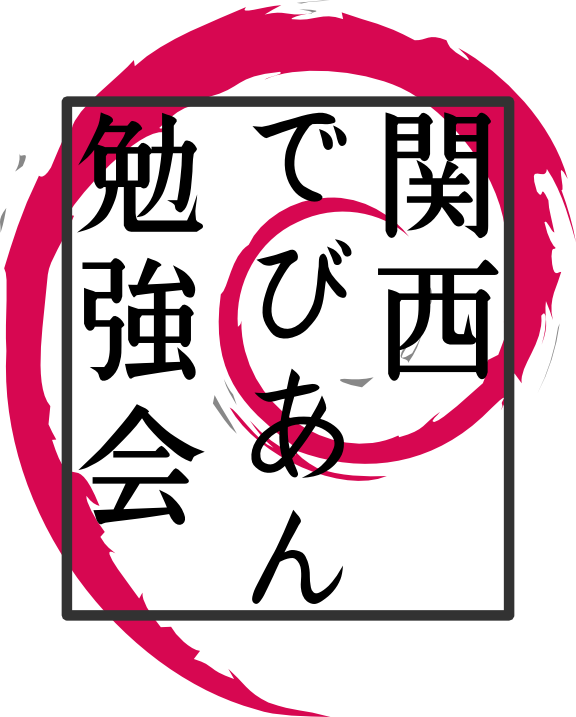
\includegraphics{image200802/kansaidebianlogo.png}
\end{center}

\begin{flushright}
\hfill{}関西 Debian 勉強会担当者 佐々木・倉敷・のがた・かわだ \\
\hfill{}\debmtgyear{}年\debmtgmonth{}月\debmtgdate{}日
\end{flushright}

\thispagestyle{empty}
\end{titlepage}

\dancersection{Introduction}{Debian JP}

 関西Debian勉強会はDebian GNU/Linuxのさまざまなトピック
 (新しいパッケージ、Debian特有の機能の仕組、Debian界隈で起こった出来事、
 などなど)について話し合う会です。

 目的として次の三つを考えています。
 \begin{itemize}
  \item MLや掲示板ではなく、直接顔を合わせる事での情報交換の促進
  \item 定期的に集まれる場所
  \item 資料の作成
 \end{itemize}

 それでは、楽しい一時をお楽しみ下さい。

\newpage

\begin{minipage}[b]{0.2\hsize}
 {\rotatebox{90}{\fontsize{80}{80}
{\gt 関西 Debian 勉強会}}}
\end{minipage}
\begin{minipage}[b]{0.8\hsize}
\hrule
\vspace{2mm}
\hrule
\setcounter{tocdepth}{1}
\tableofcontents
\vspace{2mm}
\hrule
\end{minipage}

\dancersection{最近のDebian関係のイベント報告}{Debian JP}

\subsection{第 57 回関西 Debian 勉強会}
57 回目の関西 Debian 勉強会は 3 月 25 日に開催されました。

月刊企画の Debian Policy は第5章の control ファイルについての話、t-code と konoha のパッケージ作成 2 本立ての話でした。
t-code に加えて konoha と、パッケージ作成のお話を継続して行って月刊企画にできるとよいですね。

\subsection{第 87 回東京エリア Debian 勉強会}
87 回目の東京エリア Debian 勉強会は 4 月 21 日に開催されました。

Debian での node.js 入門の話、Android OS 搭載機材に Debian をインストールする話、
月刊 Debhelper は dh\_md5sums コマンドと dh\_shtrip コマンドの話の3本立てでした。
\clearpage

\dancersection{事前課題}{Debian JP}

今回は以下の課題を出題しました.
\begin{screen}
  \begin{enumerate}
  \item Debian Policy の第2章を読んで、アーカイブエリアのmain、contrib、non-freeの違いについて説明してください。
  \item 次のうち、著作権の対象になりそうなものを選んでみよう。\\
パスワード、Linux のカーネルイメージ、Linux カーネルのソースコード、Emacs Lisp の言語仕様、動画の圧縮方式
  \end{enumerate}
\end{screen}

参加者の皆さんの解答は以下の通りです.

\begin{prework}{  清野陽一 }
  \begin{enumerate}
  \item
    \begin{description}
    \item [main]はDFSGに準拠していて、コンパイル及び実行時にmain以外のパッケージを必要としないもの。
    \item [contrib]はDFSG準拠であるが、mainと違い、コンパイル及び実行時にmain以外に属しているパッケージに依存していても良い。または非フリーなプログラムのラッパーパッケージなど。例えばgoogleearth-packageなど。
    \item [non-free]はDFSGに準拠していない、もしくは特許や法的な問題のために配布に問題のあるもの。
    \end{description}
    いずれにしてもあまりにバグだらけでサポートが拒否されるようなものは拒絶される。また、mainやcontribはマニュアルのポリシー要求に完全適合、non-freeも可能な限り準拠することが求められる。
  \item Linux カーネルのソースコード
  \end{enumerate}
\end{prework}

\begin{prework}{ 川江 }
  \begin{enumerate}
  \item 
    \begin{description}
    \item [main] フリー
    \item [contrib] non-freeに依存する部分がある
    \item [non-free] フリーでない
    \end{description}
  \item パスワード Linuxのカーネルイメージ 動画の圧縮方式
  \end{enumerate}
\end{prework}

\clearpage

\begin{prework}{ よしだともひろ }
  \begin{enumerate}
  \item
    \begin{description}
    \item [main] DFSGに準拠していて、コンパイル、実行時にmainの範囲外のパッケージを必要としないパッケージ
    \item [contrib] DFSGに準拠していて、contribまたはnon-freeに属するパッケージをコンパイル、実行時に必要とするパッケージ
    \item [non-free] DFSG に準拠していないパッケージ、または特許やその他の法的問題のために配布に問題のあるパッケージ
    \end{description}
  \item Linux のカーネルイメージ、Linux カーネルのソースコード
  \end{enumerate}
\end{prework}

\begin{prework}{ かわだてつたろう }
  \begin{enumerate}
  \item のちほど
  \item 「Linux のカーネルイメージ」と「Linux カーネルのソースコード」「Emacs Lisp の言語仕様」「動画の圧縮方式」かな。
  \end{enumerate}
\end{prework}

\begin{prework}{ 山城の国の住人 久保博 }
  \begin{enumerate}
  \item 回答1.
    \begin{description}
    \item [non-free]は、DFSG 非準拠だったり、配布に問題のあるパッケージを収める
    \item [contrib]は、DFSG 準拠で main 以外のパッケージやそれ以外のソフトウェアに依存するものを収める。
    \item [main]は、DFSG 準拠で、 main のパッケージへのみ依存するものを収める
    \end{description}
  \item 回答2\\
    会場で披露します
  \end{enumerate}
\end{prework}

\begin{prework}{ yoda }
  (無回答)
\end{prework}

\begin{prework}{ 酒井 忠紀 }
  \begin{enumerate}
  \item
    \begin{description}
    \item [main] 該当パッケージと依存パッケージ共にDFSG に準拠している
    \item [contrib] 該当パッケージは DFSG に準拠しているが、依存パッケージが準拠していない
    \item [non-free] 該当パッケージが DFSG に準拠していない
    \end{description}
  \item 著作権の対象は「思想または感情の創作的な表現」とういうことなので、以下の4つでしょうか?
    \begin{itemize}
    \item Linuxのカーネルイメージ
    \item Linuxカーネルのソースコード
    \item Emacs Lispの言語仕様
    \item 動画の圧縮方式
    \end{itemize}
        「創作的な」が何を含むのか、いまいち理解できていません。
  \end{enumerate}
\end{prework}

\begin{prework}{ yyatsuo }
  \begin{enumerate}
  \item
    \begin{description}
    \item [main] DSFG準拠で依存も含め完全に free なもの
    \item [contrib] DSFG準拠でそれ自体は free だけど non-free に依存するもの
    \item [non-free] DSFGに準拠せず、free ではないもの
    \end{description}
  \item
    \begin{description}
    \item [パスワード] "創作"かどうか微妙。性質上、個人と関連付けるものではない = ただの文字の羅列であると考えると創作ではないので著作権対象外。
    \item [カーネルイメージ] ソースコードは著作物でバイナリはその派生的著作物である、と考えれば著作権の対象。
    \item [ソースコード] (日本では)著作権保護対象
    \item [言語仕様] 仕様は著作権対象外
    \item [圧縮方式] アイディアそのものであれば著作権対象外。別の知財権で保護されるのでは?
    \end{description}
  \end{enumerate}
\end{prework}

\begin{prework}{ のがたじゅん }
  \begin{enumerate}
  \item
    \begin{description}
    \item [main] DFSGに合致したソフトウェアが収められている。
    \item [contrib] DFSGに合致しているが、DFSGに合致していないソフトウェアに依存しているソフトウェア、もしくはnon-freeなソフトウェアのラッパーなどが収められる。
    \item [non-free] DFSGに合致しない、もしくは特許や法的に問題のあるソフトウェアが収められる。
  \end{description}
  \item Linuxカーネルイメージとカーネルのソースコードかな?\\
    パスワードや言語仕様は思想や感情を創作的にあらわしたものではないし、圧縮方式は特許で守られるものだと思う。
  \end{enumerate}
\end{prework}

\begin{prework}{ 佐々木洋平 }
\begin{enumerate}
  \item 課題1の回答
  \begin{description}
    \item[main] DFSG に準拠するソフトウェア
    \item[contrib] それ自体は DFSG に準拠しているが、動作に non-free のソフトウェアが必要なソフトウェア
    \item[non-free] DFSG に準拠しないソフトウェア。
  \end{description}
  \item 課題2の回答
  \begin{description}
    \item 主張するかはともかく、これらのモンがどこからともなく湧くわけはないので、
          著作者は存在するような気がするんですがね.
  \end{description}
\end{enumerate}
\end{prework}

\begin{prework}{ 西山和広 }
  \begin{enumerate}
  \item
    \begin{description}
    \item [main] DFSG に準拠していて main だけで完結出来るパッケージを収録
    \item [contrib] DFSG に準拠しているが main 以外のものに依存しているパッケージを収録
    \item [non-free] DFSG に準拠していないパッケージやその他の配布に問題のあるパッケージを収録
    \end{description}
  \item 直感で選ぶと Linux のカーネルイメージ、Linux カーネルのソースコード だと思いました。
  \end{enumerate}
\end{prework}

\begin{prework}{ lurdan }
  \begin{enumerate}
  \item
    \begin{description}
    \item [main]には DFSG-Free なソフトウェア
    \item [non-free]には DFSG-Free ではないソフトウェア
    \item [contrib]にはそれ自体が DFSG-Free であっても、動作するために non-free なソフトウェアに依存しているもの
    \end{description}
    がそれぞれ収録されます
  \item Linux カーネルイメージ\\
    Linux カーネルのソースコード
  \end{enumerate}
\end{prework}

\clearpage
%% -*-tex-*-
%%
%% Copyright (C) 2012 Hiroshi Kubo  all rights reserved.
%% 本資料の著作権は、著者である久保博 <h-kubo@geisya.or.jp> にあります。
%%
%% This document material is licensed under the GNU General Public License version 2.0.
%% This document is originally in the form of LaTeX source code. This shall be referenced as the ``Corresponding Source''
%% Any compiled forms including DVI, Postscript, and PDF from the original source code shall be reference as the ``Object code''.
%%
\dancersection{フリーソフトウェアと戯れるための著作権入門}{山城国の住人 久保博}


\subsection{前書き}

人生のいきがかり上、割と最近になって著作権の勉強を始めることになりました。
法律の専門家ではありませんので、自信を持っての発表ではないですが、
みなさんと一緒に考えていくきっかけになればと思います。

\subsection{はじめに}

日本を含む多くの国で、ソフトウェアは、生み出された時から著作権という権利の対象になっています。

ですから、フリーソフトウェアも、生まれた時から誰かのもの、ということになっています。
フリーであっても誰かのものである、という点では、登記された土地は空き地であっても誰かのものであるのとにているかも知れません。

フリーソフトウェアの精神は、一介の利用者が自分自身のためにソフトウェアを使うことを
妨げるようなことは最大限避けるようにしていますから、自分自身のためにフリーソフトウェアを使う限り、
知らなくても困ったことにはなりません。

でも、そこから一歩踏み出そうとすれば、誰かのものであるということを尊重することが求められることになります。
この要請は、著作権法と、それを前提とする契約に基づいています。

そこで、Debian Project が配布しているようなフリーソフトウェアを扱う場面をいくつか想定して、
そこに著作権と契約がどのように関わってくるのか、解き明かしてみます。なお、日本の著作権法を元にしてお話します。



\subsection{知的財産権}

ソフトウェアが誰かのものである、とは、どういうことでしょう。

知的な作業を通して創り出された、無体物(プログラムを含む)には、
創り出した人の努力や労力に報いるために、さまざまな制度を定める法律が整備されています。
その中でも、知的な創造によってつくり出された無体物に対して、
財産権の対象となる有体物の物権に良く似た権利を設定する仕組みが法律で定められています。
この物権に似た権利を知的財産権といいます。
そして、知的財産権は、創造した人あるいは登録した人が享受する権利なのです。

これが、ソフトウェアが誰かのものである、ということの、現代社会における意味です。

ソフトウェアが関係する知的財産権には、次のものがあります。

\begin{itemize}
\item[{\bf{著作権}}] 「思想又は感情を創作的に表現したものであつて、文芸、学術、美術又は音楽の範囲に属するもの」に対する独占的な保護をもたらす権利
\item[{\bf{特許権}}]  発明(自然法則を利用した技術的思想の創作のうち、高度なもの)を登録することによって独占的な保護をもたらす権利
\item[{\bf{実用新案権}}] 考案(自然法則を利用した技術的思想の創作)を登録することによって独占的な保護をもたらす権利
\item[{\bf{意匠権}}] 意匠(物品の形状、模様若しくは色彩またはこれらの結合であって、視覚を通じて美感を起こさせるもの)を登録することによって独占的な保護をもたらす権利
\item[{\bf{商標権}}] 商標を登録することによって独占的な保護をもたらす権利
\end{itemize}

プログラムそのものは、著作権の対象になります。
また、プログラムで実装されたアルゴリズムは特許や実用新案の保護の対象になり得る場合がありますし、プログラムの名称やロゴは商標としての保護の対象になり得ます\footnote{Debian も電子計算機などの指定商品での商標登録がされており、登録番号は 第4595288号です。ちなみに、指定商品「菓子、パン」で「デビアン」という称呼の登録番号第1708032号の登録商標があります。面白いですね。}。
GUIの画面のデザインは海外では意匠登録の対象となり得る場合もあるようですが、日本では今のところ対象ではありません。

この中でも、ソフトウェアについて一番よく問題になるのは、著作権です。

\subsection{著作権}
\subsubsection{著作権の性質}

正確ではないですが端的に言えば、著作権法は、著作物を作った人に著作物に対する独占的な権利を与える法律です。
その著作権法で定められている著作権には次のような性質があります。

\begin{itemize}
\item 著作物を作ったら、発生します。
\item 著作物を公表しなくても発生します。
\item (特許と違って、)役所に登録しなくても発生します\footnote{このような権利の発生のさせ方を無方式主義と言います。なお、かつてアメリカは、無方式主義ではありませんでした。}。
\item 著作物が生まれてから、著作者の死後50年間、著作権の保護は続きます。
\item 他人が著作物を勝手に利用した場合、差止請求権、損害賠償請求権を行使するという方法で対抗できます\footnote{著作権法第百十四条に基づいて損害額を推定しても、フリーソフトウェアの場合、0円にしかならないですが…。}。
\end{itemize}
ですから、新しいプログラムが作られれば、必ずと言っていいほど著作権が関係してきます。

逆に言えば、著作物をパブリックドメインとするためには、著作権を放棄する手続きなどが必要になるわけです。
また、著作物を利用するには、著作権者から利用許諾をもらうべし、というのが著作権法に則った正しい方法です。

したがって、ソフトウェアとともに
\begin{itemize}
\item 著作権に基づく利用許諾契約書
\item 著作権を放棄する宣言あるいは放棄済であることの明示的な説明
\end{itemize}
のどちらかを手に入れないと、著作権法に違反していない確信を持ってソフトウェアを使うことが難しい、ということになります。
Debian Project は、社会契約\cite{DebianSocialContract}に基づいて行動しており、この点に関して厳密に考えてパッケージを作っているわけです。

\subsubsection{著作権の存続期間}

権利が有効である時間の範囲を存続期間と言います。

「著作者が死んでも著作権の保護が続くってどういうこと?」と不思議に思うかも知れませんね。
 著作権は相続できるのです。相続する人があれば、続くんです。
相続を含めて、権利を引き継ぐことを「承継」と言います。
承継する人がなければ、著作権は消滅します。

\par
\begin{center}
\fbox{
\parbox{0.8\linewidth}{
\begin{center}{\Large\bf 筆者からお願い!}\\
あなたが作って公開しているプログラム、\linebreak[1]あなたの死後に誰が著作権を相続するか予め周りの人に教えておいて下さい。
\end{center}
}
}
\end{center}
\par


なお、FSF\footnote{Free Sofware Foundation. ウェブサイトは {\url http://www.fsf.org/}}は、FSFへ著作権を譲渡することを勧めています\cite{FSFassign}。著作者の死後、GPL\footnote{GNU General Public License}で公開したフリーソフトウェアの行く末を託すこともできますね\footnote{著作権の譲渡に関しては、日本の著作権法には第三者対抗要件に登録が必要などの難しい話が関係するので、筆者はどうしたらいいのか、理解できていません。}。

\subsubsection{著作権の内訳}

著作権とは、権利の束みたいなものです。著作物を利用する方法などによって、細かい権利が定められています。

それらは大別すると、「著作人格権」と「著作財産権」に分かれ、それぞれの下に次のような権利が条文で定められています。

\begin{description}
\item[著作人格権]「公表権」「氏名表示権」「同一性保持権」
\item[著作権(著作財産権)]「複製権」「上演権」「演奏権」「上映権」「公衆送信権」「伝達権」「口述権」「展示権」「頒布権」「譲渡権」「貸与権」「翻訳権」「翻案権」「二次的著作物の利用に関する権利 」
\end{description}

この中には、ソフトウェアが関係しないものもあります。

\subsection{Debian Project が配布しているものの何が著作物?}

さて、著作物とはどんなものがあるか、著作権法を読んでみると、次のようなことが書いてあります。

著作物とは、「思想又は感情を創作的に表現したものであつて、文芸、学術、美術又は音楽の範囲に属するものをいう。」
(著作権法第二条)


更に、著作権法では、例を挙げて著作物を定義しています。

\begin{verbatim}
第十条 この法律にいう著作物を例示すると、おおむね次のとおりである。
  	一 小説、脚本、論文、講演その他の言語の著作物
  	二 音楽の著作物
  	三 舞踊又は無言劇の著作物
  	四 絵画、版画、彫刻その他の美術の著作物
  	五 建築の著作物
  	六 地図又は学術的な性質を有する図面、図表、模型その他の図形の著作物
  	七 映画の著作物
  	八 写真の著作物
  	九 プログラムの著作物

2 事実の伝達にすぎない雑報及び時事の報道は、前項第一号に掲げる著作物に該当しない。

3 第一項第九号に掲げる著作物に対するこの法律による保護は、その著作物を作成するために用いるプログラム言語、規約及び解法に及ばない。この場合において、これらの用語の意義は、次の各号に定めるところによる。
  	一 プログラム言語 プログラムを表現する手段としての文字その他の記号及びその体系をいう。
  	二 規約 特定のプログラムにおける前号のプログラム言語の用法についての特別の約束をいう。
  	三 解法 プログラムにおける電子計算機に対する指令の組合せの方法をいう。
\end{verbatim}

ということで、プログラムは、プログラム著作物です。オブジェクトコードもプログラム著作物である、という判例もあるようです\footnote{東京地判昭和60年3月8日判タ 561号 169頁「ディグダグ」事件 という判例があるそうです\cite{saito}。}。

また、Debian Project が配布するものにはプログラム以外にも、文章、写真画像、地図データなどありますが、著作物です。


\subsection{著作権を踏まえた Debian Project からの配布物とのおつき合い}


\subsubsection{著作権のことを気にせずに Debian のシステムをインストールしました。何かまずいことをしていないでしょうか?}

自分で使う目的でインストールしたのですよね?

インストールする前に利用許諾契約を読んで、同意して、それからインストールするのが理想的ですが、そうでない場合もよくあるかと思います。

Debian Project が配っているインストーラーを使って普通にインストールしたなら、
インストールしたソフトウェアの利用許諾契約に同意したことにしましょう。
インストーラーでインストールしたソフトウェアはすべて DFSG\footnote{The Debian Free Software Guidelines\cite{DFSG}} に準拠しているので、ほとんどあなたは不利益を被っていません。

\begin{itemize}
\item 金銭的な対価は要求されません。
\item 使うだけなら無償の貢献も要求されません。
\item あなたの某かの権利を放棄したり断念したり譲渡したりすることもありません。
\end{itemize}

なにか気をつけることがあるとすれば、免責条項くらいでしょうか。

 ほぼすべてのフリーソフトウェアの利用許諾では、その動作に関して無保証で、免責条項が盛り込まれています\footnote{フリーでなくても、無保証である場合が多いですし、保証はあっても賠償額の上限をソフトウェア購入代金とすることも珍しくありません。}。
無保証であることに関する同意は、ほとんどのソフトウェアが採用している利用許諾の契約の条項の一部です。同意できないなら、利用する権利はありません。

したがって、著作者に対して、次に掲げることについて何の文句をつける筋合いもありません。
\begin{itemize}
\item  期待通りに動かない
\item  そもそも動かない
\item  ソフトウェアを使ったせいで、地位や財産を失った
\item  ソフトウェアを信じたせいで、地位や財産を失った
%%\item  ソフトウェアを使ったせいで、心が傷ついた
\end{itemize}

%% ここで BTS の話を一席
でも、多くのフリーソフトウェアの開発元や Debian Project には、バグ報告の窓口がありますね。
あれは、義務でやっているのでないのです。大いなる親切以外の何物でもありません。


%% \subsubsection{知合いのパソコンに Debian のシステムをインストールしました。}

%% そのパソコンを利用する持ち主の方に、利用許諾書に同意してもらいましょう。
%% 別に、書類に判子をつくような手続きは必要ありません。

%% 全部を理解してもらうのはなかなか困難だとは思いますが、
%% 自分のために使って、うまくいかなくても作者の方々に文句をいう筋合いはないことに納得してもらえれば実際上は十分です。


\subsubsection{Debian のフリーソフトウェアを使わないけど配ります。}

ちょっと待って! あなたは、著作者と契約を結ばなくてはなりません!

著作権には「複製権」「自動公衆送信権」「送信可能化権」という権利が含まれているのです。
極めて簡単に分かりやすくいうと
\begin{description}
\item[複製権 ] 簡単にいうと、コピーする権利。
\item[自動公衆送信権] 公衆に送信する権利。
\item[送信可能化権] 公衆がアクセスしてダウンロードできるサーバーに著作物を置く権利。
\end{description}
です。
著作者が独占的に保持する権利ですから、あなたは、ソフトウェアを配ったり、公開されているサイトにアップロードする前には、著作者の許可が必要です。


でも実は、Debian アーカイブの main セクションと contrib セクションに含まれるソフトウェアのソースコードを
{\em そのまま}無料で配布する場合は、利用許諾に同意する必要はあるものの、
実質的には何らかの義務や制約に縛られることはありませんので、
ほとんど気にかける必要はないです。

というのも、main と contrib に含まれるソフトウェアは、すべて DFSG\cite{DFSG} に準拠してます。
DFSG に準拠しているこということは、ソースコードの自由な配布が利用許諾契約上、認められていることになるのです。

これに対して、バイナリパッケージを配布する場合は、配布先でソースコードが手に入れることができるように配慮しないといけないライセンスが多いです\footnote{GPL や LGPL (GNU Lesser General Public License)  が典型的な例です。}。
ソースコードが入手できるような配布を強制することで、ソフトウェアの自由を担保しようとしているわけです。
注意しましょう。


また、利用許諾の内容を理解する前に、適当に一部を削ったり、一部を抜き出して配らないようにしましょう。
というのも、著作権には「同一性保持権」という権利があります。
勝手に削ることも含めて、著作物を勝手に改変することは著作権法が禁じています。
改変に際しては許諾が必要で、許諾された範囲での改変しか許されません。

幸い、 DFSG準拠なら改変は許されますし、改変されたソフトウェアの複製を配布することも許されますが、
契約毎に許されるための条件はあります。

それから、勝手に著作者の氏名を削ってはいけません。
「氏名表示権」を侵害することになります。

\par\begin{center}{\Large そのまま配るのが一番無難です。}\end{center}

\subsubsection{Debian をインストールされてるパソコンをもらいました}

一般的に、正規の方法で入手したソフトウェアを手元にコピーを残さずに誰かに譲り渡すことは構わないのですが、
パソコンをもらっただけでは、そのパソコンにインストールされているソフトウェアを無条件に使っていいことにはなりません。
くれた人は「好きにしていいよ」と言ってくれていても、利用許諾の契約には同意して利用しましょう。

物品の譲渡と一緒に著作権の利用許諾がなされたとみなせる場合というのは、
特別に著作権法に明記されています\footnote{美術品の展示権など。}。
原則として、物品の譲渡とそこに宿っている著作物の利用許諾とは、別ものなのです。

ちなみに、ソフトウェアの利用許諾書にはしばしば non-transferable という言葉で、
利用権の譲渡を明示的に禁止する文言が現れますが、その場合は、契約上利用権を譲渡できないことになっています。

\subsection{特許との関係}

利用許諾書には、著作権ではない別の知的財産権に基づく利用許諾が含まれる場合があります。
よく使われる「ライセンス」と言う言葉に含まれる、利用許諾の根拠になる権利は著作権だけとは限らないわけです。

例えば、DFSG準拠の利用許諾の中には、特許に関する条項が含まれているものがあり、
その代表的なものには、 Apache License 2.0 と、 GPL 3.0 があります。

この二つの利用許諾には、ともに、「ソースコードの貢献者が保有する特許のうち、ある範囲のものは、無償で利用を許諾する、」という趣旨の条項が含まれています。
Apache License 2.0 は、貢献者が自分の貢献したコードに含まれる特許を利用許諾するのに対し、
 GPL 3.0 では、貢献者が配布したコードに含まれる特許を利用許諾する点が違います。


\subsection{その他関係する法律}

最後に、ソフトウェアが関係しそうな法律をいくつか挙げておきます。

\begin{itemize}
\item 不正アクセス禁止法
\item 不正競争防止法
\item 刑法のいわゆるウィルス作成罪
\item 関税法
\item 民法
%% \item PL法
\end{itemize}


\subsection{宿題}

次の問題に答えてみましょう。

\begin{itemize}
\item 「アルゴリズム体操」の振付けは、著作権法第十条の何の著作物でしょうか?
\item GCC (GNU Compiler Collection) は、プログラムの著作物として保護されるでしょうか?
\item 著作権(著作財産権)のうち、ソフトウェアに関係あるものを挙げてみましょう。
\item かつて特許によって自由な配布が制限されたソフトウェアがありました。どんなものがあるか、調べてみましょう。
\end{itemize}



\subsection{まとめ}


フリーソフトウェアに関わる著作権の仕組みを簡単に解説しました。

\begin{thebibliography}{99}
    \bibitem{DebianSocialContract} Debian 社会契約,
                    \url{http://www.debian.org/social\_contract}

    \bibitem{DFSG} The Debian Free Software Guidelines,
    \url{http://www.debian.org/social\_contract\#guidelines}

    \bibitem{CopyrightLaw} 著作件法 ,
                    {\url http://law.e-gov.go.jp/htmldata/S45/S45HO048.html}

    \bibitem{FSFassign} なぜFSFは貢献者に著作権の譲渡をお願いしているのか {\url http://www.gnu.org/licenses/why-assign.html}

    \bibitem{GPLv3chikujou} GPLv3 逐条解説
      \url{http://ossipedia.ipa.go.jp/DL/doc/187/5/0904/ON/}

    \bibitem{saito} 著作権法 , 斉藤博, 2000年, 有斐閣

\end{thebibliography}
\clearpage

\dancersection{スクリプティング言語 Konoha の Debian パッケージ化について}{酒井 忠紀}
\subsection{はじめに}
前回は Konoha の概要説明と その Debian パッケージの内容確認をしました。
今回は、以下について説明します。
\begin{itemize}
\item upstream との調整経緯
\item debian/rules 修正とパッケージ分割について
\end{itemize}

\subsection{upstream との調整経緯}
\subsubsection{ライセンス問題について}
前回、ご指摘を頂いた以下のライセンス問題を upstream の方に報告しました。
\begin{itemize}
\item Web サイトでは GPLv3 と記述されているが、配布物の COPYING ファイルは LGPLv3 になっている
\item 配布物の中に "third-party" というディレクトリがあり、その中に jar ファイルや Apache Linense 2.0 ライセンスのソースの tar アーカイブがある
\end{itemize}

現在、ライセンスに関しては upsteam 側で再検討を行っているようです。

また、"Konoha Non-Disclosure License 1.0" とは、有償サポート付きのライセンスを検討していたということでした。

\begin{itembox}[l]{質問}
  \begin{enumerate}
  \item ユーザの視点から、扱いやすいライセンスの組み合わせなどはありますでしょうか?\\
    GPLv2 or Later と New BSD のデュアルライセンスなど
  \item 言語によって相性の良いライセンスなどがありますでしょうか?\\
    例えば、Qt は言語バインディングによって以下のようにライセンスが異なるようです。
    \begin{itemize}
    \item Ada ... GPL
    \item C++ ... LGPL
    \item C\# \& .NET(qt4dotnet) ... LGPL
    \item Java ... LGPL
    \item Lisp ... BSD
    \item Lua ... MIT
    \item Perl ... GPL
    \item PHP ... LGPL
    \item Python(PyQt) ... GPL
    \item Ruby ... LGPL
    \item Tcl ... GPL
    \end{itemize}
  \end{enumerate}
\end{itembox}

\subsubsection{upstream の Konoha 開発状況について}
現在公開されている Konoha は Konoha 1.0 ですが、upsteam では試作的な扱いとなっているようです。

正規のものは現在開発中の Konoha 2.0 になり、6月頃のリリースを目標に作業が進められているようです。

upstream において、Konoha 1.0 はもうサポートする気がないようなので、ITP するのは Konoha 2.0 がリリースされてからにしようと考えています。

また、Debian 7.0(Wheezy) への新規パッケージの取り込みは 6月で閉じてしまうので、時期的に断念し、次の Debian 8.0? を目標にしようと考えています。

\subsubsection{Konoha 2.0 について}
現在開発中の Konoha 2.0 について、特徴を簡単に説明します。

\begin{enumerate}
\item 最小限の構文\\
  if, int, String, void, boolean, array, 関数定義 のみサポートする。(代入がない)\\
  POSIX lowlevel bind と呼ばれている。
\item Konoha Assignment\\
  言語のシンタックスをスクリプトで追加できる。
\item ライブラリ\\
  既存の Konoha 1.0 の機能は、ライブラリとして提供する。\\
  必要な機能のみ、インポートして使用できる。
\item 言語バインディング\\
  C, Java, JavaScript, C\#, その他を検討している。
\item ドキュメントの自動生成
\end{enumerate}

Konoha 2.0 は、以下に記述する4つのモジュールから構成されます。
\begin{itemize}
\item konoha (コマンド本体)
\item sugar (パーサー)
\item gc (Garbage Collection)
\item vm (Virtual Machine)
\end{itemize}

バイナリサイズが 約1/10 (100KB) になったので、組み込み機器やアプリケーションなどに容易に組み込むことが可能になるようです。

\subsection{debian/rules 修正とパッケージ分割について}
Konoha 2.0 はまだ公開されていないので、Konoha 1.0 のままになりますが、前回指摘を受けた以下の2つを修正しました。

\subsubsection{debian/rules 修正}
前回は debhelper を使用して記述していましたが、今回は dh を使用して記述し直しました。

記述内容をかなり省略することができ、行数が 43行 から 7行 になりました。
(コメントと空行は除く)

修正した debian/rules を以下に記述します。
\begin{commandline}
#!/usr/bin/make -f
# -*- makefile -*-
# Uncomment this to turn on verbose mode.
#export DH_VERBOSE=1

%:
        dh $@ --buildsystem cmake --builddirectory=build

override_dh_auto_configure :
        dh_auto_configure -- -DCMAKE_INSTALL_PREFIX=/usr -DMPI_ROOT_DIR=/usr/lib/openmpi -DUSE_QT4=ON -DK_REVISION=961

override_dh_auto_test :

\end{commandline}
%$ for emacs font-lock

--buildsystemオプションで、ビルドシステムに cmake を指定しました。
前回は configure ターゲットを自前で記述していました。

ビルドシステムは、以下が指定できるようです。
\begin{itemize}
\item autoconf ... GNU Autoconf (configure)
\item perl\_makemaker ... Perl MakeMaker (Makefile.PL)
\item makefile ... simple Makefile
\item python\_distutils ... Python Distutils (setup.py)
\item perl\_build ... Perl Module::Build (Build.PL)
\item cmake ... Cmake (CmakeLists.txt)
\item ant ... Ant (build.xml)
\end{itemize}

--builddirectoryオプションで、ビルドディレクトリを指定しました。
前回は configure, build, clear, install ターゲットで、'cd build \&\&' を記述していました。

override\_dh\_auto\_configure ターゲットで、cmake のオプションをオーバライドしました。

override\_dh\_auto\_test ターゲットで、make test を実行しないようにしました。

debian/rules の書き方は、以下を参考にしました。\\
\url{http://www.debian.org/doc/manuals/packaging-tutorial/packaging-tutorial.pdf}\\
\url{http://kitenet.net/~joey/talks/debhelper/debhelper-slides.pdf}

\subsubsection{パッケージ分割}
前回はシングルパッケージにしていましたが、Debian ポリシーに従い、以下の3つのパッケージに分割しました。

\begin{itemize}
\item konoha パッケージ (実行バイナリ)\\
  konoha\_1.0.0+svn961-1\_amd64.deb
\item libkonoha1 パッケージ (ライブラリ + シンボリックリンク(SONAME))\\
  libkonoha1\_1.0.0+svn961-1\_amd64.deb
\item konoha-dev パッケージ (ヘッダファイル + シンボリックリンク)\\
  konoha-dev\_1.0.0+svn961-1\_amd64.deb
\end{itemize}

konoha パッケージ と konoha-dev パッケージは、libkonoha1 パッケージに依存するように定義しました。

修正した debian/control を以下に記述します。
ruby1.9.1 のソースパッケージを参考にしました。
\begin{commandline}
Source: konoha
Section: interpreters
Priority: optional
Maintainer: Tadaki SAKAI <stadaki.dev@gmail.com>
Build-Depends: debhelper (>= 7.0.50~), cmake, libffi-dev, libmemcached-dev, libsqlite3-dev, libqt4-dev,
  libqt4-opengl-dev, libqtwebkit-dev, libcairo2-dev, libopenmpi-dev, libjson0-dev, libcurl4-nss-dev,
  libxml2-dev, openjdk-6-jdk, ant, libreadline-dev
Standards-Version: 3.9.3
Homepage: http://konoha.sourceforge.jp/
Vcs-Svn: http://konoha.googlecode.com/svn/trunk/
Vcs-Browser: http://code.google.com/p/konoha/downloads/list

Package: konoha
Architecture: amd64
Depends: libkonoha1 (= ${binary:Version}), ${shlibs:Depends}, ${misc:Depends}
Suggests: konoha-dev
Description: Interpreter of statically-typed scripting language Konoha
 Konoha scripting language has a Java-like syntax, multiplatform
 virtual machine, and static typing system.

Package: libkonoha1
Section: libs
Architecture: amd64
Depends: ${shlibs:Depends}, ${misc:Depends}
Description: Libraries necessary to run Konoha
 Konoha scripting language has a Java-like syntax, multiplatform
 virtual machine, and static typing system.

Package: konoha-dev
Architecture: amd64
Depends: libkonoha1 (= ${binary:Version}), ${shlibs:Depends}, ${misc:Depends}
Recommends: konoha (= ${binary:Version})
Description: Header files for compiling extension modules for the Konoha
 Konoha scripting language has a Java-like syntax, multiplatform
 virtual machine, and static typing system
\end{commandline}
%$ for emacs font-lock


konoha パッケージ でインストールするファイルは debian/konoha.install で定義しました。\\
debian/konoha.install を以下に記述します。
\begin{commandline}
debian/tmp/usr/bin/*
\end{commandline}

libkonoha1 パッケージ でインストールするファイルは debian/libkonoha1.install で定義しました。\\
 debian/libkonoha1.install を以下に記述します。
\begin{commandline}
debian/tmp/usr/lib/libkonoha.so.1.0
debian/tmp/usr/lib/libkonoha.so.1.0.0
debian/tmp/usr/konoha/*
\end{commandline}

konoha-dev パッケージ でインストールするファイルは debian/konoha-dev.install で定義しました。\\
debian/konoha-dev.install を以下に記述します。
\begin{commandline}
debian/tmp/usr/include/*
debian/tmp/usr/lib/libkonoha.so
\end{commandline}

\subsection{Konoha 1.0 Debian パッケージの作成手順}

sid で以下の実行する。
\begin{commandline}
$ sudo apt-get install cmake libffi-dev libmemcached-dev \
libsqlite3-dev libqt4-dev libqt4-opengl-dev libqtwebkit-dev \
libcairo2-dev libopenmpi-dev libjson0-dev libcurl4-nss-dev \
libxml2-dev libreadline-dev openjdk-6-jdk ant
$ svn export http://konoha.googlecode.com/svn/trunk/ konoha-read-only
$ cd konoha-read-only
$ tar cvfz konoha.tar.gz konoha
$ mv konoha konoha-1.0.0+svn961
$ cd konoha-1.0.0+svn961
$ dh_make --copyright gpl3 --file=../konoha.tar.gz
\end{commandline}
%$ for emacs font-lock
前章に記述した内容で、以下のファイルを編集する。\\
(copyright, changelog に関しては、第57回関西 Debian 勉強会の資料を参照。)
\begin{commandline}
  debian/rules
  debian/control
  debian/konoha.install
  debian/libkonoha1.install
  debian/konoha-dev.install
  debian/copyright
  debian/changelog
\end{commandline}
ビルドを実行。
\begin{commandline}
$ debuild -us -uc
\end{commandline}
%$ for emacs font-lock

親ディレクトリに以下が作成される。
\begin{commandline}
libkonoha1_1.0.0+svn961-1_amd64.deb
konoha-dev_1.0.0+svn961-1_amd64.deb
konoha_1.0.0+svn961-1_amd64.deb
konoha_1.0.0+svn961-1.dsc
konoha_1.0.0+svn961.orig.tar.gz
konoha_1.0.0+svn961-1.debian.tar.gz
konoha_1.0.0+svn961-1_amd64.build
konoha_1.0.0+svn961-1_amd64.changes
\end{commandline}

lintian では、まだ Warning などが出力されています。
ITP number や、man ファイル、Konoha Extra Package の格納位置などを修正する必要があります。

\clearpage

\dancersection{月刊 Debian Policy 第3回 「Debian アーカイブ」}{かわだ てつたろう}

諸般の事情で今回の担当となりました かわだ です。

今回読むのは第2章の「Debian のアーカイブ」についてです。
Debian Policy はパッケージについて書かれているわけですが、この章ではパッケージの集りであるアーカイブをどのように管理、配布するのかについて説明されています。
Debian Policy は読んだことの無い方でも Debian を使っていれば聞いたことのある内容でしょう。

さて、事前課題で内容は読んで理解していただいていると思いますのでざっと内容をみていきましょう。

\subsection{Debian フリーソフトウェアガイドライン}
Debian がフリーであると考えるソフトウェアの定義です。原文の Debian Free Software Guidelines を略した DFSG という単語もよく使われます。
「DFSG フリー」や「DFSG に準拠」という言い方はこのガイドラインに準拠したソフトウェアである、Debian が認めるフリーなソフトウェアであるということです。

DFSG は Debian 社会契約\footnote{http://www.debian.org/social\_contract}の一部であり Debian の根幹ですので一度じっくりと読んでみてください。

\subsection{アーカイブエリア}
\subsubsection{main}
Debian ディストリビューションといえばこの main アーカイブエリアのことを指します。

main に収録されるパッケージは DFSG に準拠していなければならず、コンパイル時や実行時にアーカイブエリア外のソフトウェアを必要としないこと、メンテナンスできること、Debian Policyに適合していることが求められます。

このアーカイブエリアのパッケージは誰でも自由\footnote{http://www.debian.org/intro/free}に使用、共有、修正、配布することができます。

\subsubsection{contrib}
contrib アーカイブエリアには、DFSG に準拠しているがコンパイル時や実行時にアーカイブエリア外のソフトウェアを要求するため main アーカイブエリアに置けないパッケージが収録されます。

\subsubsection{non-free}
non-free アーカイブエリアには、DFSG に準拠しないか配布に問題があるパッケージが収録されています。このアーカイブエリアのパッケージは自由に使用、共有、修正、配布することができません。

\subsection{著作権に関する考慮}
著作権について疑義があるソフトウェアはアーカイブに収録されることが留保されます。また、著作権が明示されていない作品の配布や変更は{\large 認められていません}ので注意してください。

パッケージは著作権情報と配布ライセンスの無修正コピーを /usr/share/doc/{\it package}/copyright ファイルとして同封し配布しなければなりません。


\subsection{セクションとプライオリティ}
セクションは Debian アーカイブメンテナによって公式に提供されており、勝手に追加することはできません。

プライオリティは高い順に required、important、standard、optional、extra があり、大半のパッケージは optional に属します。
また、プライオリティの高いパッケージはビルド時を除いてプライオリティの低いパッケージに依存してはいけません。

\begin{itembox}[l]{プライオリティ}
\begin{description}
\item [required] システムが適切に機能するために必要なパッケージ
\item [important] Unix ライクなシステムに必ず入っていることが期待されるプログラムのパッケージ
\item [standard] ほどよく小規模ながらキャラクタベースのシステムを提供するパッケージ
\item [optional] インストールしておく価値のある全てのパッケージ
\item [extra] 上記いずれかが指定されているパッケージと衝突するパッケージ
\end{description}
\end{itembox}


\subsection{最近の変更点}
日本語訳版がある Version 3.9.1.0 から Version 3.9.3.1 までに加えられた変更点を押さえておきましょう。

Version 3.9.2.0
\begin{itemize}
\item 「Debian GNU/Linux ディストリビューション」が「Debian ディストリビューション」と改められました。
\item main、contrib、non-free アーカイブエリアとは、が追記されています。
\end{itemize}

Version 3.9.3.0
\begin{itemize}
\item main アーカイブエリアのパッケージがアーカイブエリア外のパッケージを必要とする(required)だけでなく推奨する(recommend)ことも明記されました。
  ("Depends"、"Recommends"、"Build-Depends" に加えて "Pre-Depends" と "Build-Depends-Indep" が明記されています。)
\item セクションに education、introspection、metapackages の3つが追加されました。
\end{itemize}

\subsection{最後に}
次回の月刊 Debian Policy は。。。

\clearpage

\dancersection{今後の予定}{Debian JP}

\subsection{次回}

次回は、2012年5月27日に福島区民センターで行います。\\
発表については未定ですので、みなさまの発表をお待ちしております。

次々回は、2012年6月23日(土)に京都大学で大統一Debian勉強会\footnote{\url{http://gum.debian.or.jp}}を行ないます。

% 冊子にするために、4の倍数にする必要がある。
% そのための調整
\dancersection{メモ}{}
\mbox{}\newpage
\mbox{}\newpage

\printindex
 \cleartooddpage

 \begin{minipage}[b]{0.2\hsize}
  \rotatebox{90}{\fontsize{80}{80} {\gt 関西 Debian 勉強会} }
 \end{minipage}
 \begin{minipage}[b]{0.8\hsize}

 \vspace*{15cm}
 \rule{\hsize}{1mm}
 \vspace{2mm}
 
\includegraphics[width=2cm]{image200502/openlogo-nd.eps}
 \noindent \Large \bf Debian 勉強会資料\\ \\
 \noindent \normalfont \debmtgyear{}年\debmtgmonth{}月\debmtgdate{}日 \hspace{5mm}  初版第1刷発行\\
 \noindent \normalfont 関西 Debian 勉強会 (編集・印刷・発行)\\
 \rule{\hsize}{1mm}
 \end{minipage}

\end{document}
